\begin{figure}[b!]
  \vspace{-1.5em}
  \centering
  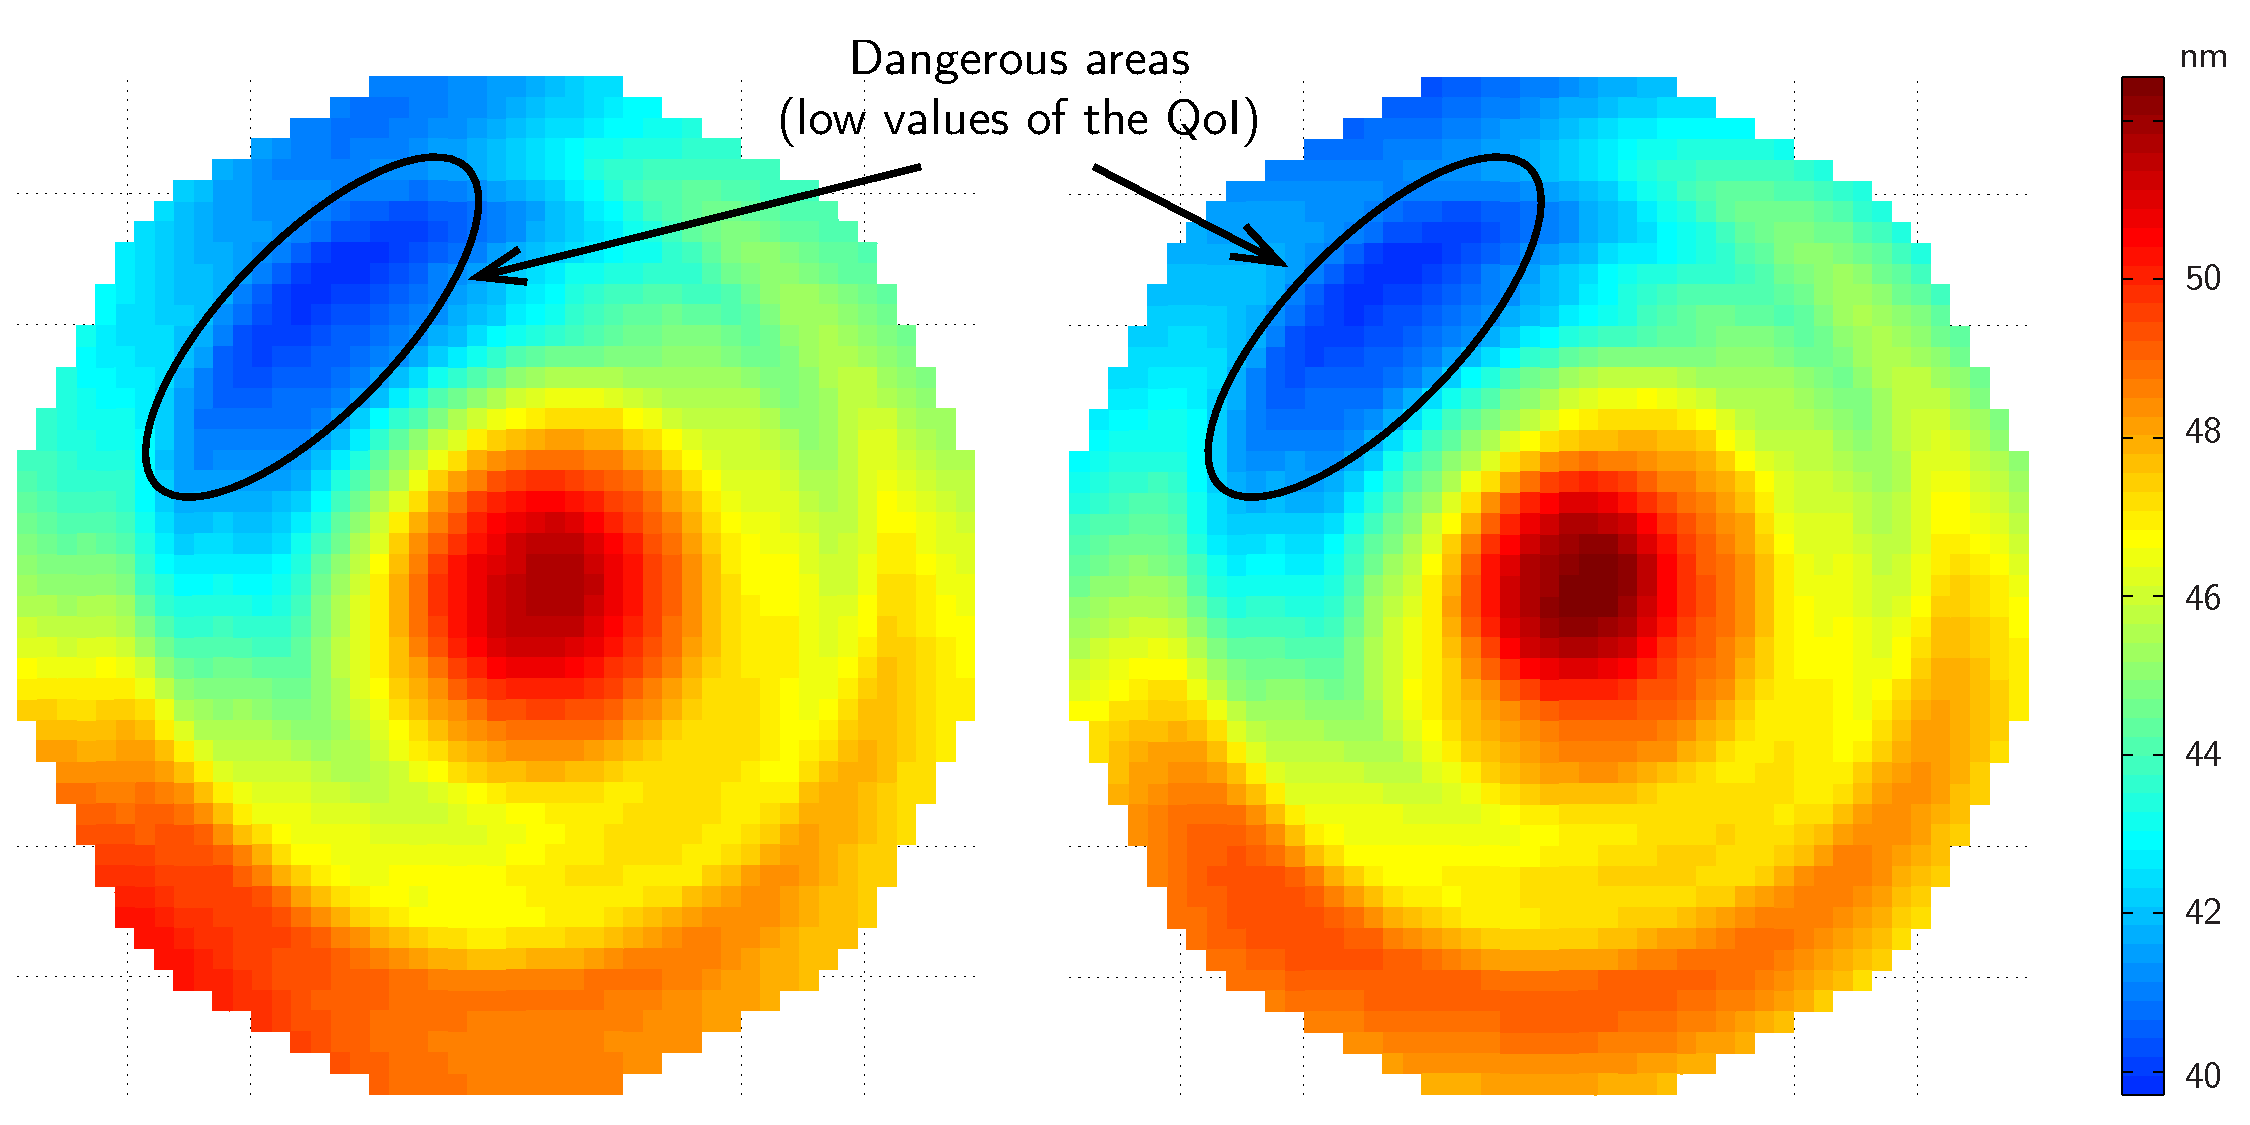
\includegraphics[width=1\linewidth]{include/assets/wafer-qoi.pdf}
  \caption{The true (on the left) and inferred (on the right) distribution of the QoI across the wafer.}
  \flabel{wafer-qoi}
\end{figure}

Let us consider an important application of the proposed technique: the characterization of the distribution, across a silicon wafer, of the effective channel length, denoted by $\u$. The effective channel length has one of the strongest effects on the subthreshold leakage current and, consequently, on power and temperature \cite{juan2012}; at the same time, $\u$ is well-known to be severely deteriorated by process variation \cite{chandrakasan2001, srivastava2010}.
Assume the technological process imposes a lower bound $\u_*$ on $\u$.\footnote{For simplicity, a possible upper bound on the effective channel length is ignored in the motivational example.} This bound separates defective dies ($\u < \u_*$) from those that are acceptable ($\u \geq \u_*$).
In order to reduce costs, the manufacturer is interested in detecting the faulty dies and taking them out of the production process at early stages.
Then the possible actions that they might take with respect to a single die on the wafer are: (a) keep the die if it conforms to the specification; (b) recycle the die otherwise.
Let the distribution of $\u$ across the wafer be the one depicted on the left side of \fref{wafer-qoi}.
The gradient from navy to dark red represents the transition of $\u$ from low to high values; hence, the navy regions have a high level of the power and heat dissipation.\footnote{The experimental setup will be described in detail in \sref{experimental-results}.}

In order to quantify the uncertainty due to the variability of the effective channel length $\u$, one can find the above-mentioned distribution by removing the top layer of (thus, destroying) the dies and measuring $\u$ directly.
Alternatively, despite the fact that the knowledge of $\u$ is more preferable, one can step back and decide to characterize process variation using some other parameter that can be measured without the need of damaging the dies, \eg, the leakage current.
It should be noted that, in this case, the chosen surrogate is the final product, and $\u$ is left unknown.
In either way, adequate test structures have to be present on the dies in order to take the corresponding measurements.
The problem, however, is that the described procedure is technologically complex and, thus, might significantly increase the production costs.
Moreover, the first approach implies that the measured dies have to be recycled afterwards, and the second implies that the design decisions will be based on a surrogate quantity instead of the primary source of uncertainty, which can compromise the reliability of such decisions.

Our technique works differently.
In order to characterize the effective channel length $\u$, we monitor an auxiliary quantity $\q$ that depends on $\u$ and is more advantageous from the measurement perspective.
The distribution of $\u$ across the whole wafer is then obtained via Bayesian inference \cite{gelman2004} applied the collected measurements of $\q$.
These measurements are taken only on a small number of locations on the wafer and can potentially be corrupted by the noise due to the imperfection of the measurement equipments.

Assume that $\q$ is temperature.
We can then apply a fixed workload to a few dies on the wafer and measure the corresponding temperature profiles.
Since temperature does not require extra equipments to be deployed on the wafer and can be tracked using infrared cameras \cite{mesa-martinez2007} or built-in facilities of the dies, our approach can reduce the costs associated with the analysis of process variation.
The result of our framework applied to a set of noisy temperature profiles measured for only 7\% of the dies on the wafer is shown on the right side of \fref{wafer-qoi}, and the locations of the selected dies are depicted in \fref{wafer-measured}.
It can be seen that the two maps in \fref{wafer-qoi} closely match each other implying that our approach is able to reconstruct the distribution of the effective channel length with a high level of accuracy.

Another feature of the proposed framework is that probabilities of various events, \eg, $\probabilityMeasure(\u \geq \u_*)$, can readily be estimated.
This is important since, in reality, the true values are unknown for us (otherwise, we would not need to quantify them), and, therefore, we can rely on our decisions only up to a certain probability.
We can then reformulate the decision rule defined earlier as follows: (a) keep the die if $\probabilityMeasure(\u \geq \u_*)$ is larger than a certain threshold; (b) recycle the die otherwise.
An illustration of this rule is given in \fref{wafer-defective} where the lower bound $\u_*$ is set to two standard deviations below the mean value of the effective channel length; the probability threshold of the action (a) is set to 0.9; the crosses mark both the true and inferred defective dies (they coincide); and the gradient from light gray to red corresponds to the inferred probability of a die to be defective. It can be seen that the inference accurately detects faulty regions.
\begin{figure}
\begin{minipage}{0.45\linewidth}
  \centering
  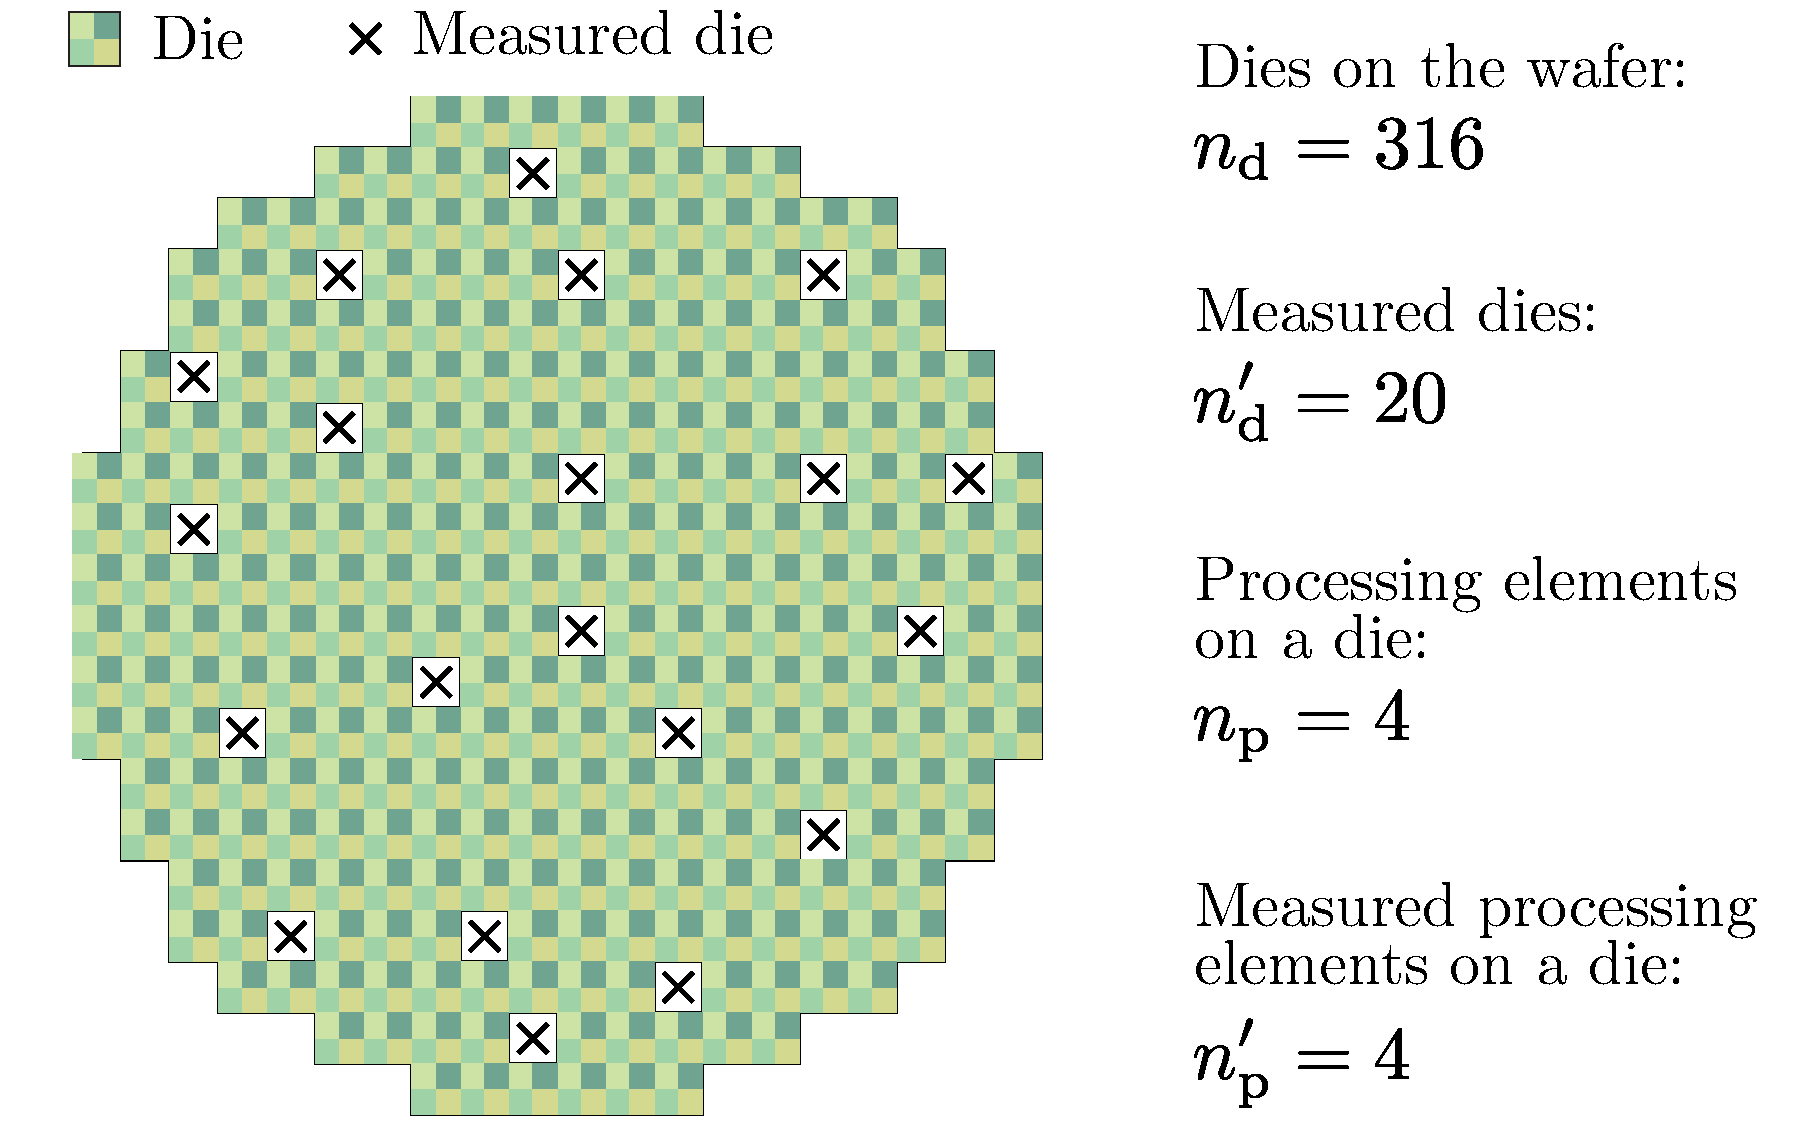
\includegraphics[width=1\linewidth]{include/figures/wafer-measured.pdf}
  \vspace{-1.5em}
  \caption{Measurements.}
  \flabel{wafer-measured}
\end{minipage}
\begin{minipage}{0.55\linewidth}
  \vspace{0.1em}
  \centering
  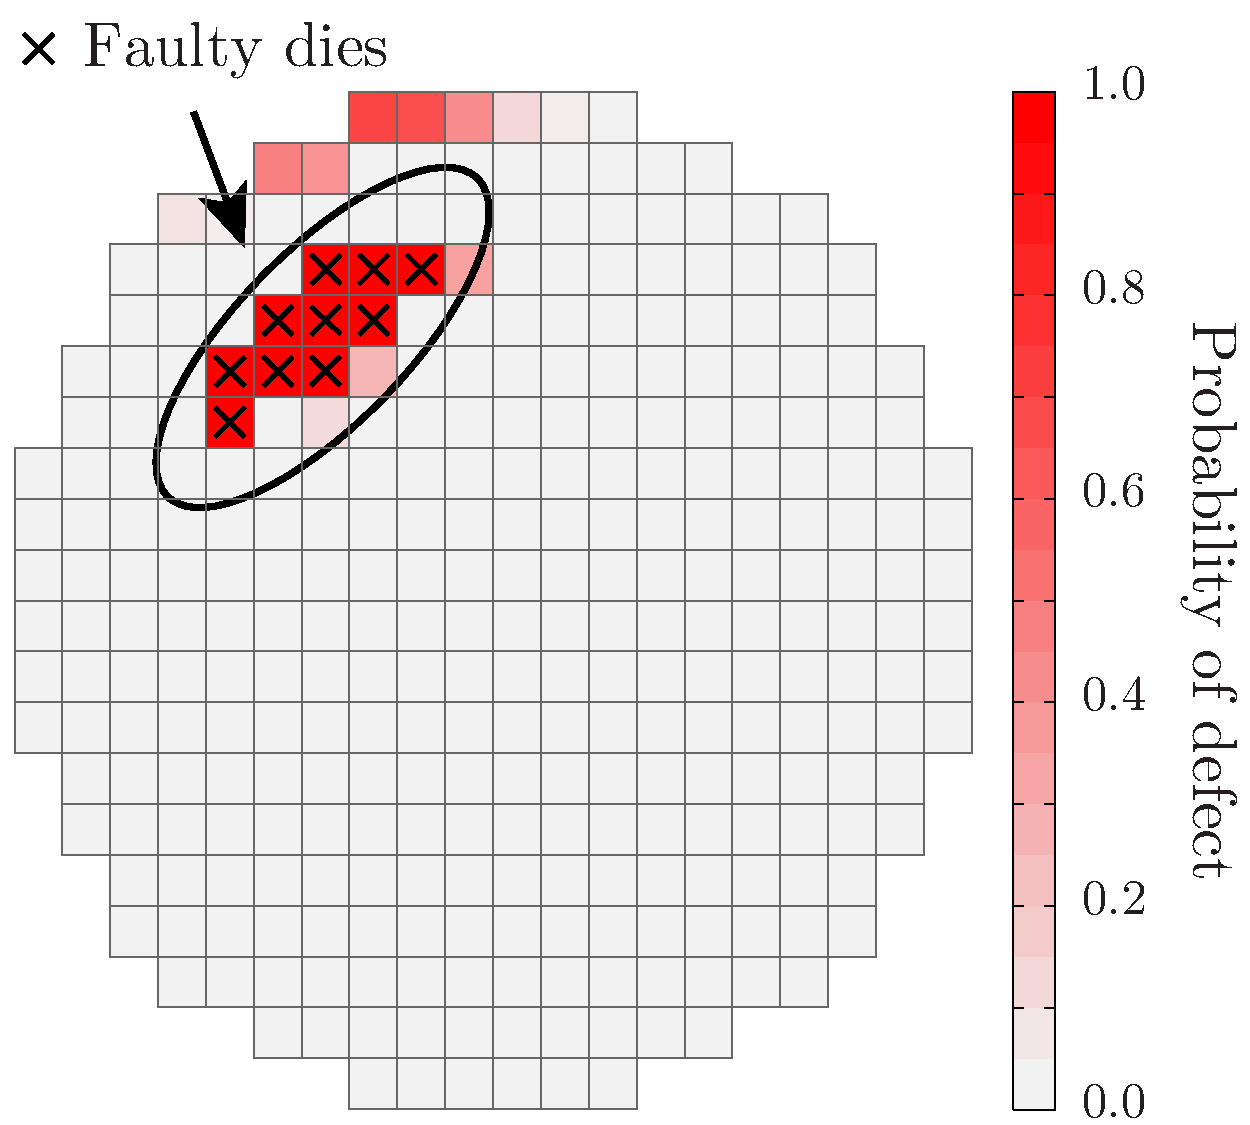
\includegraphics[width=1\linewidth]{include/figures/wafer-defective.pdf}
  \vspace{-1.5em}
  \caption{Probability of defect.}
  \flabel{wafer-defective}
\end{minipage}
\vspace{-1.5em}
\end{figure}


In addition, we can introduce a trade-off action: (c) expose the die to a thorough inspection (\eg, via a test structure) if $\probabilityMeasure(\u \geq \u_*)$ is smaller than the threshold of (a) and is larger than some other threshold, \eg, $0.1 < \probabilityMeasure(\u \geq \u_*) < 0.9$. In this case, we can reduce costs by examining only those dies for which there is neither sufficiently strong evidence of their satisfactory nor unsatisfactory condition.
Furthermore, one can take into consideration a so-called utility function, which, for each combination of an outcome of $\u$ and a taken action, returns the gain that the decision maker obtains.
For example, such a function can favor a rare omission of malfunctioning dies to a frequent inspection of correct dies as the latter might involve much more costs.
The optimal decision is given by the action that maximizes the expected utility with respect to both the observed data and prior knowledge on $\u$.
Thus, all possible $\u$ weighted by their probabilities will be taken into account in the final decision, incorporating also the preferences of the user via the utility function.

Finally, we would like to emphasize that temperature is just one option.
In certain situations, it might be preferable to perform the above inference based on measurements of some other auxiliary quantity $\q$ provided that it depends on the one that we wish to characterize, \ie, on $\u$.
For example, $\q$ can be the leakage current, which can be readily measured if adequate test structures have already been deployed on the wafer for other purposes.
